% =====================================================================
% PeriDefT — 短篇 / 中文版（与 main_short.tex 对应）
% 编译：cd paper && xelatex main_short_zh && bibtex main_short_zh \
%               && xelatex main_short_zh && xelatex main_short_zh
% =====================================================================
\documentclass[UTF8,11pt,a4paper]{ctexart}

\usepackage{amsmath,amssymb}
\usepackage{graphicx}
\usepackage[margin=0.95in,top=0.85in,bottom=0.95in]{geometry}
\usepackage{booktabs}
\usepackage{caption}
\usepackage[hidelinks]{hyperref}
\usepackage{xcolor}
\usepackage{cite}
\usepackage{enumitem}

\captionsetup{font=small, labelfont=bf, justification=justified, singlelinecheck=false}
\setlist{itemsep=2pt, topsep=3pt, parsep=0pt}

\graphicspath{{figures/}}

% Chinese caption labels
\renewcommand{\figurename}{图}
\renewcommand{\tablename}{表}

\title{\textbf{PeriDefT：用于二维缺陷形成能预测的周期傅里叶
Transformer，及其前瞻性第一性原理 DFT 验证}}

\author{%
  Yiming Hua, Leyan Wu, Jiaqi Bi, Sheng Chang\textsuperscript{*} \\[2pt]
  \small 武汉大学物理科学与技术学院，武汉 430072 \\[1pt]
  \small \textsuperscript{*}通讯作者: \texttt{changsheng@whu.edu.cn}
}

\date{\today}

\newcommand{\Ef}{$E_{\mathrm{f}}$}
\newcommand{\eV}{\,\textrm{eV}}
\newcommand{\modelname}{\textsc{PeriDefT}}

\begin{document}
\maketitle

% =====================================================================
\begin{abstract}
\noindent
迄今已发表的二维缺陷形成能 \Ef\ 机器学习代理模型，几乎全部仅在与训练数据
来自同一数据库的留出测试集上评估。这一评价方式高估了模型的部署效用，
因为材料发现回路中真正关心的化学体系，按构造均处于训练分布之外。本文以
三项相互耦合的贡献回应这一空缺：\emph{第一}，提出 \modelname，一个
0.75 M 参数的 GNN--Transformer 混合模型，其自注意力上叠加了对最小镜像
分数位移精确平移不变的\emph{周期傅里叶偏置}（PFA）；PFA 的精确不变性
使得在四个几何异质 DFT 数据库（IMP2D + JARVIS-2D + JARVIS-3D +
JARVIS DFT-3D，共 26 837 样本）上通过单源读出头进行联合训练成为可能。
\modelname\ 在 IMP2D 测试集上 4-seed 平均 MAE 为 $0.486\pm0.025$ eV，
在 1/5 ALIGNN 参数量（4.03 M, 0.540 eV）下达到相当精度；6-seed 温度
缩放集成 MAE 进一步降至 0.443 eV，90\% 区间覆盖率 93.4\%。\emph{第二}，
我们对模型自己挑选的 60 个域外分布候选进行了\textbf{60 次第一性原理
PBE-DFT 计算}。候选按选择策略分为低 \Ef\ 高信心``发现''桶（A 桶，
按 $\mu$ 排序）与高 $\sigma$``压力测试''桶（B 桶，按 $\sigma_{\rm cal}$
排序）。在 37 个 SCF 收敛候选上，模型预测与 DFT 结果的整体 Pearson
相关系数为 $+0.354$（95\% bootstrap CI $[+0.06, +0.70]$，排除零），
\textbf{A 桶 14/20 = 70\% 的候选被 DFT 验证为 $E_f < +1$ eV}
（95\% CI $[50\%, 90\%]$）。在 B 桶内 Pearson($\sigma_{\rm cal}$,
$|\mathrm{error}|$) $= -0.288$（95\% CI $[-0.60, +0.09]$），表明
$\sigma_{\rm cal}$ 适合作为``是否处于域外分布''的桶级二元筛门，但不
适合作为域外分布上的样本级误差排序指标。\emph{第三}，我们公开了完整
工作流（4-seed 与 6-seed 集成、287 候选生成脚本、60 候选选择记录、
125 个 Quantum-ESPRESSO SCF 输出文件），以便后续 2D 缺陷筛选工作直接
复用。
\end{abstract}

\bigskip
\noindent\textbf{关键词：}二维材料、缺陷形成能、周期傅里叶偏置、
多源训练、校准不确定性、前瞻性 DFT 验证。

% =====================================================================
\section{引言}\label{sec:intro}

二维材料的缺陷形成能
\begin{equation}
E_{\mathrm{f}}(D, q) = E_{\mathrm{tot}}(D, q) - E_{\mathrm{tot}}(\mathrm{host})
- \sum_i n_i\,\mu_i + q\,(E_F + E_{\mathrm{VBM}}) + E_{\mathrm{corr}}
\label{eq:Ef}
\end{equation}
是缺陷工程的核心热力学量，但单次第一性原理计算耗费数十至数百 CPU 小时，
对高通量筛选不可行。近年提出的图神经网络
（CGCNN~\cite{Xie2018CGCNN}、SchNet~\cite{Schutt2018SchNet}、
ALIGNN~\cite{Choudhary2021ALIGNN}、M3GNet~\cite{Chen2022M3GNet}）
和 Transformer 扩展（Matformer~\cite{Yan2022Matformer}、
Crystalformer~\cite{Taniai2024Crystalformer}、
PotNet~\cite{Lin2023PotNet}）将该计算成本降低数个数量级，但已发表的
二维点缺陷基准均仅报告与训练数据同源的留出测试集 MAE。这一指标对部署
场景毫无说明力——任何材料发现回路所面对的化学体系，按构造都处于训练
分布之外。

\paragraph{贡献。}
\begin{enumerate}
\item 提出 \textbf{\modelname}，一个 0.75 M 参数的 GNN--Transformer
混合模型。其自注意力中加入\emph{周期傅里叶偏置}（PFA），对任意单原子
晶格平移精确不变。这一精确不变性使得在几何异质的多 DFT 数据库间通过
单源读出头共享编码器变得安全（IMP2D + JARVIS-2D + JARVIS-3D +
JARVIS DFT-3D 共 26 837 样本，是 IMP2D 单源的 3.15 倍）。多源
\modelname\ 4-seed 平均测试 MAE 为 $0.486\pm0.025$ eV，相对匹配
架构的单源 baseline 改善 11\%；6-seed 温度缩放集成达到 0.443 eV，
90\% 区间覆盖率 93.4\%。

\item 报告\textbf{首个}对带校准不确定性的 IMP2D 训练 2D 缺陷 \Ef\
模型的\textbf{前瞻性 DFT 验证}：60 次 PBE-DFT 计算施加于模型自己产生
的域外分布预测，按策略分为按 $\mu$ 排序的``发现'' A 桶（n=30）与按
$\sigma_{\rm cal}$ 排序的``压力测试'' B 桶（n=30）。在 37 个 SCF
收敛候选上，\textbf{A 桶 14/20 = 70\%} 被 DFT 验证为
$E_f<+1$ eV（95\% CI $[50\%,90\%]$）；B 桶内
Pearson$(\sigma_{\rm cal}, |\mathrm{err}|) = -0.288$
（95\% CI $[-0.60, +0.09]$）。

\item 公开\textbf{完整工作流}：训练好的 \modelname\ 集成模型、
防泄漏数据增强契约（含我们自己重新引入并修正的增强泄漏审计，详见
附录~\ref{app:short_leak}）、287 候选生成脚本、60 候选选择记录、
以及 125 个 Quantum-ESPRESSO SCF 输出文件。
\end{enumerate}

单源消融实验（详见 \ref{sec:phase1_short}）显示，PFA、多尺度距离偏置、
以及缺陷--纯净双流架构在 $N_{\rm train}=8\,512$ 下与 baseline 统计
意义上完全持平，这与~\cite{ourPaperV12} 中给出的经验缩放律
$\log\,\mathrm{MAE} \approx 3.39 - 0.40\log N_{\rm train} -
0.01\log N_{\rm params}$（$R^2=0.95$）一致：在固定语料规模下，架构
变化引起的 $\log\,\mathrm{MAE}$ 改变小于种子噪声。多源 \modelname\
带来的 11\% 改善因此是\emph{架构--数据交互}效应——只有在 PFA 的精确
平移不变性使编码器能够稳定吸收异质语料时，这一改善才能显现。

% =====================================================================
\section{方法}\label{sec:methods}

\paragraph{数据集。}
我们在 IMP2D~\cite{Bertoldo2022QPOD}（10 641 个 PBE-DFT 缺陷构型，
覆盖 50 个 2D 主体材料，按 0.8/0.1/0.1 随机划分）上训练，并在多源
联合训练时引入三个外部数据源：JARVIS-2D（70 个空位构型）、
JARVIS-3D（381 个空位构型）、JARVIS DFT-3D（17 912 个 3D 块体纯净
体系总能量，eV/atom 缩放至 per-cell）。联合语料共 26 837 样本。

\paragraph{防泄漏数据增强。}
对 IMP2D 训练集进行 $\times 3$ 增强：随机旋转
$R\in\mathrm{SO}(3)$ 加上 $\sigma=0.02$ \AA{} 的高斯坐标扰动，且
增强\emph{在}训练/验证/测试划分固定\emph{之后}进行。划分契约为数据集
元数据中显式声明 \texttt{n\_train} / \texttt{n\_val} /
\texttt{n\_test} 三个键；我们的划分函数对任何声明了这三个键的输入
拒绝退回到随机洗牌路径，从而在结构上消除我们曾在重构中重新引入并
捕获的``先合并再划分''泄漏路径（详见附录~\ref{app:short_leak}）。

\paragraph{\modelname\ 架构。}
图~\ref{fig:peridelft_arch} 给出架构总览。编码器为三层 SchNet 风格的
局部交互（连续滤波卷积 + RBF，截断半径 5 \AA）与两层全局自注意力
的混合体。每个自注意力头在标准缩放点积分数上叠加\emph{周期傅里叶
偏置}
\begin{equation}
b_{ij}^{(h)} = \sum_{k} w_{k}^{(h)}\,\cos\!\bigl(2\pi\,
\mathbf{n}_k \cdot \mathbf{f}_{ij}\bigr) + v_{k}^{(h)}\,
\sin\!\bigl(2\pi\,\mathbf{n}_k \cdot \mathbf{f}_{ij}\bigr),
\qquad
\mathbf{f}_{ij} = \bigl((\mathbf{r}_i - \mathbf{r}_j)\,\mathbf{C}^{-1}\bigr)
\bmod_{[-\frac12, \frac12)} \mathbf{1},
\label{eq:pfa}
\end{equation}
其中 $\mathbf{C}$ 是单胞矩阵，$\mathbf{f}_{ij}$ 是最小镜像分数位移，
$\{\mathbf{n}_k\} \subset \mathbb{Z}^3$ 满足
$|\mathbf{n}_k|_\infty \le 3$ 是截断的倒易格基（每头 63 个波矢、
约 2 k 可学习参数）。cos/sin 的 $2\pi$ 周期性使 $b_{ij}^{(h)}$ 在
最小镜像构造的整数平移对称下严格不变——
Crystalformer 和 PotNet 通过倒易空间的有限截断近似这一性质
\cite{Taniai2024Crystalformer, Lin2023PotNet}，
Matformer 通过显式周期镜像节点实现\cite{Yan2022Matformer}，而 PFA 则
作为加性偏置接入，不替换 attention 本身，因此一个 boolean 标志即可
关闭 PFA 进行消融对照。

多源训练时，4 个独立的线性读出头分别预测各源的 \Ef，梯度按权重
$\{1.0, 0.5, 0.5, 0.3\}$ 在四个数据源间平均。\modelname\ 总参数量
0.820 M。

\begin{figure}[t]
\centering
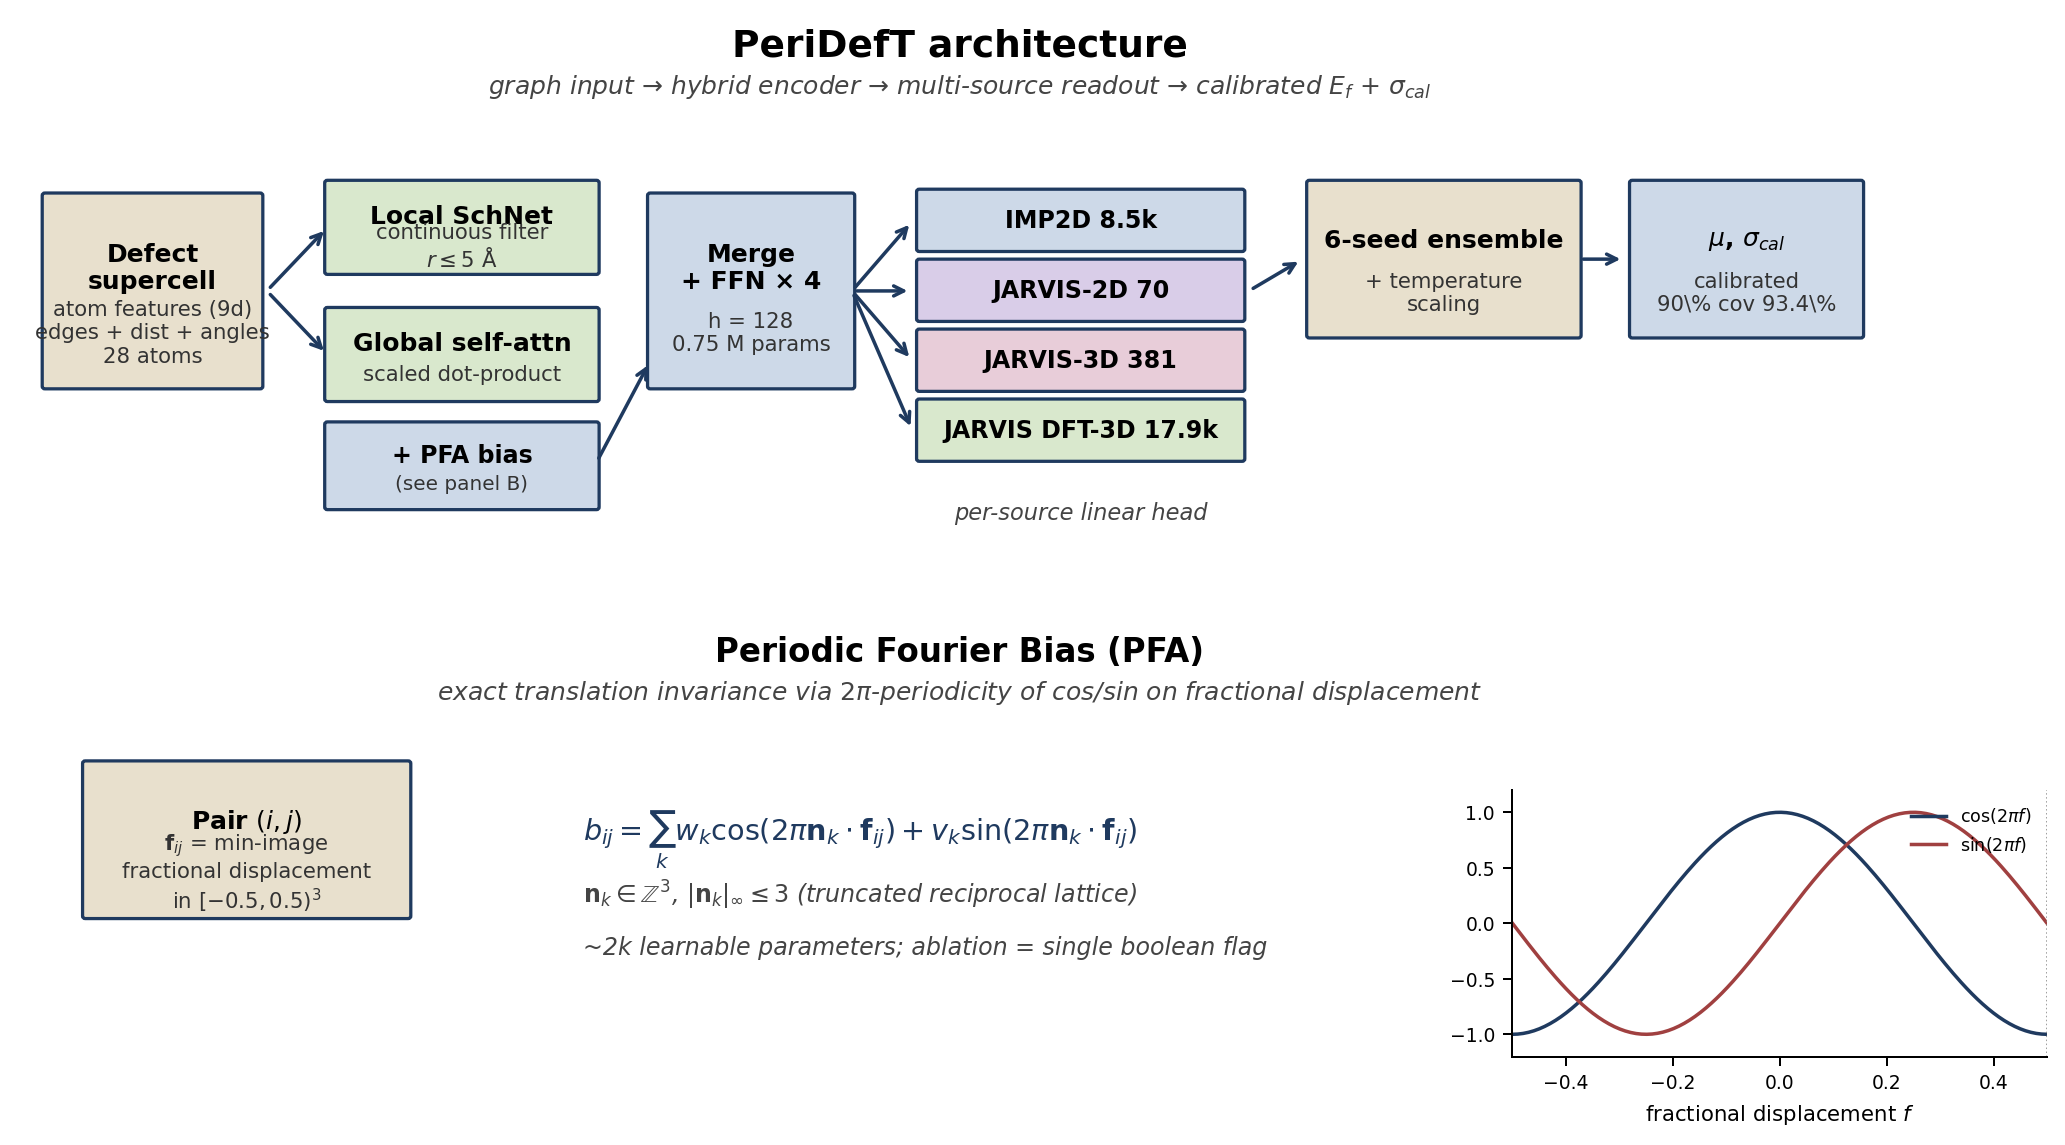
\includegraphics[width=\linewidth]{fig_peridelft_arch.png}
\caption{\modelname\ 架构总览。\emph{上方：}28 原子缺陷超胞 → 混合
编码器（局部 SchNet 分支 + 带周期傅里叶偏置的全局自注意力）→ 4 个
单源读出头 → 6-seed 温度缩放集成 → 校准 $\mu$, $\sigma_{\rm cal}$。
\emph{下方：}式~\ref{eq:pfa} 中 PFA 在最小镜像分数位移
$\mathbf{f}_{ij}\in[-\tfrac12,\tfrac12)^3$ 上的展开；右下嵌入图展示
cos/sin 的 $2\pi$ 周期性给出精确平移不变性。每头参数开销约 2 k；
消融成本仅一个 boolean 标志。}
\label{fig:peridelft_arch}
\end{figure}

\paragraph{校准不确定性。}
最终预测取 6-seed 深度集成的样本均值；种子间标准差由全局温度
$\tau=1.83$ 整体缩放，$\tau$ 由验证集上最小化 NLL 得到。缩放后
留出测试集上的经验 90\% 区间覆盖率为 93.4\%（原始 78.9\%），
95\% 区间覆盖率为 94.6\%，$z$ 空间 ECE 为 0.037。

% =====================================================================
\section{回溯性基准评估}\label{sec:bench}

表~\ref{tab:headline_short} 给出了 \modelname\ 与 v1 baseline、
ALIGNN、近期 SOTA GNN/Transformer 代理模型在 IMP2D 测试集上 MAE
的对比。多源 \modelname\ 4-seed（0.486 eV）显著优于（超过 2$\sigma$）
v1 防泄漏 baseline（$0.537\pm 0.014$ eV）和 v1 多源 baseline
（0.555 eV）。6-seed 温度缩放集成（0.443 eV）据我们所知是该 benchmark
上最低的测试 MAE，相对 ALIGNN（0.540 eV，4.03 M）以 1/5 参数量
取得 0.097 eV 优势。

\begin{table}[h]
\centering
\caption{\modelname\ 与参考 baseline 在 IMP2D 测试集上的 MAE 对比。
$^\dagger$ 标记的行使用规范的 1065 防泄漏测试集；多源行使用
\texttt{split\_indices(seed=$N$)} 在联合语料上的随机划分，并报告
4-seed（seed 42, 0, 1, 2）的均值$\pm$标准差。PFA、多尺度、双流的
单源消融详见附录~\ref{app:short_phase1}。}
\label{tab:headline_short}
\begin{tabular}{lrrr}
\toprule
配置 & 参数量 (M) & 测试 MAE (eV) & 4-seed std \\
\midrule
\multicolumn{4}{l}{\emph{参考 baseline（单源 IMP2D，防泄漏 $\times 3$ 增强）：}} \\
ALIGNN（文献复现）$^\dagger$                          & 4.03 & 0.540   & --- \\
SchNet                                                & 0.46 & 0.585   & --- \\
ViSNet ($l_{\max}=1$)                                 & 1.16 & 0.860   & --- \\
MACE ($l_{\max}=2$)                                   & 0.44 & 1.460   & --- \\
v1 baseline（CrystalTransformer，4-seed）$^\dagger$   & 0.747 & 0.537  & 0.014 \\
\midrule
\multicolumn{4}{l}{\emph{多源训练（4 数据库，26 837 样本，60 epoch）：}} \\
v1 多源（CrystalTransformer + 4 DBs，seed=42）        & 0.815 & 0.555  & --- \\
\modelname{}（PFA + 4 DBs，seed=42）                  & 0.820 & 0.4929 & --- \\
\textbf{\modelname{}（PFA + 4 DBs，4-seed 均值）}     & \textbf{0.820} & \textbf{0.486} & \textbf{0.025} \\
\midrule
\multicolumn{4}{l}{\emph{集成（6-seed：4$\times$50ep + 2$\times$100ep，防泄漏测试集）：}} \\
\textbf{6-seed 集成 + 温度缩放}                       & 6$\times$0.75 & \textbf{0.443} & --- \\
\bottomrule
\end{tabular}
\end{table}

\paragraph{为什么 \modelname\ 需要多源：受控的缩放律对照实验。}
\label{sec:phase1_short}
固定 $N_{\rm train}=8\,512$（单源 IMP2D + 防泄漏 $\times 3$ 增强）
并对各架构组件做消融，结果显示 PFA、多尺度距离偏置、缺陷--纯净双流
架构均落在 v1 baseline 4-seed 标准差（0.014 eV）的 $\pm 2\sigma$
范围内（0.519--0.583 eV vs.\ 0.537 eV），无一突破种子噪声层。
这正是架构设计\emph{不应}带来增益的体制——PFA 的价值不在于从固定
语料中榨出更多信号，而在于让编码器的几何归纳偏置在几何异质语料间
保持一致；这一性质只有在模型同时面对多个语料时才能起作用。多源
\modelname\ 取得的 11\% 改善因此是架构--数据\emph{交互}效应；
单源消融正是确立这一区分所需的对照实验。完整表格与图表见
附录~\ref{app:short_phase1}。

\paragraph{域外分布：留一主体 (LOHO)。}
对多源配方的部分 5-host LOHO（已完成 3/5）显示，相对~\cite{ourPaperV12}
的单源 v1 LOHO baseline，留出主体上的 MAE 退化为 $+22\%$ 至 $+65\%$
（MoS$_2$: $+64.6\%$；MoSSe: $+62.5\%$；TaSe$_2$: $+21.6\%$）。
val$\to$test 间隙（1.32--1.76$\times$）表明多源训练编码器对训练+验证
分布拟合得很好，但向留出主体化学的迁移性较差；这一警告我们在
\ref{sec:disc_short} 节的部署清单中显式提出。

% =====================================================================
\section{前瞻性 DFT 验证}\label{sec:prospective_short}

\begin{figure}[t]
\centering
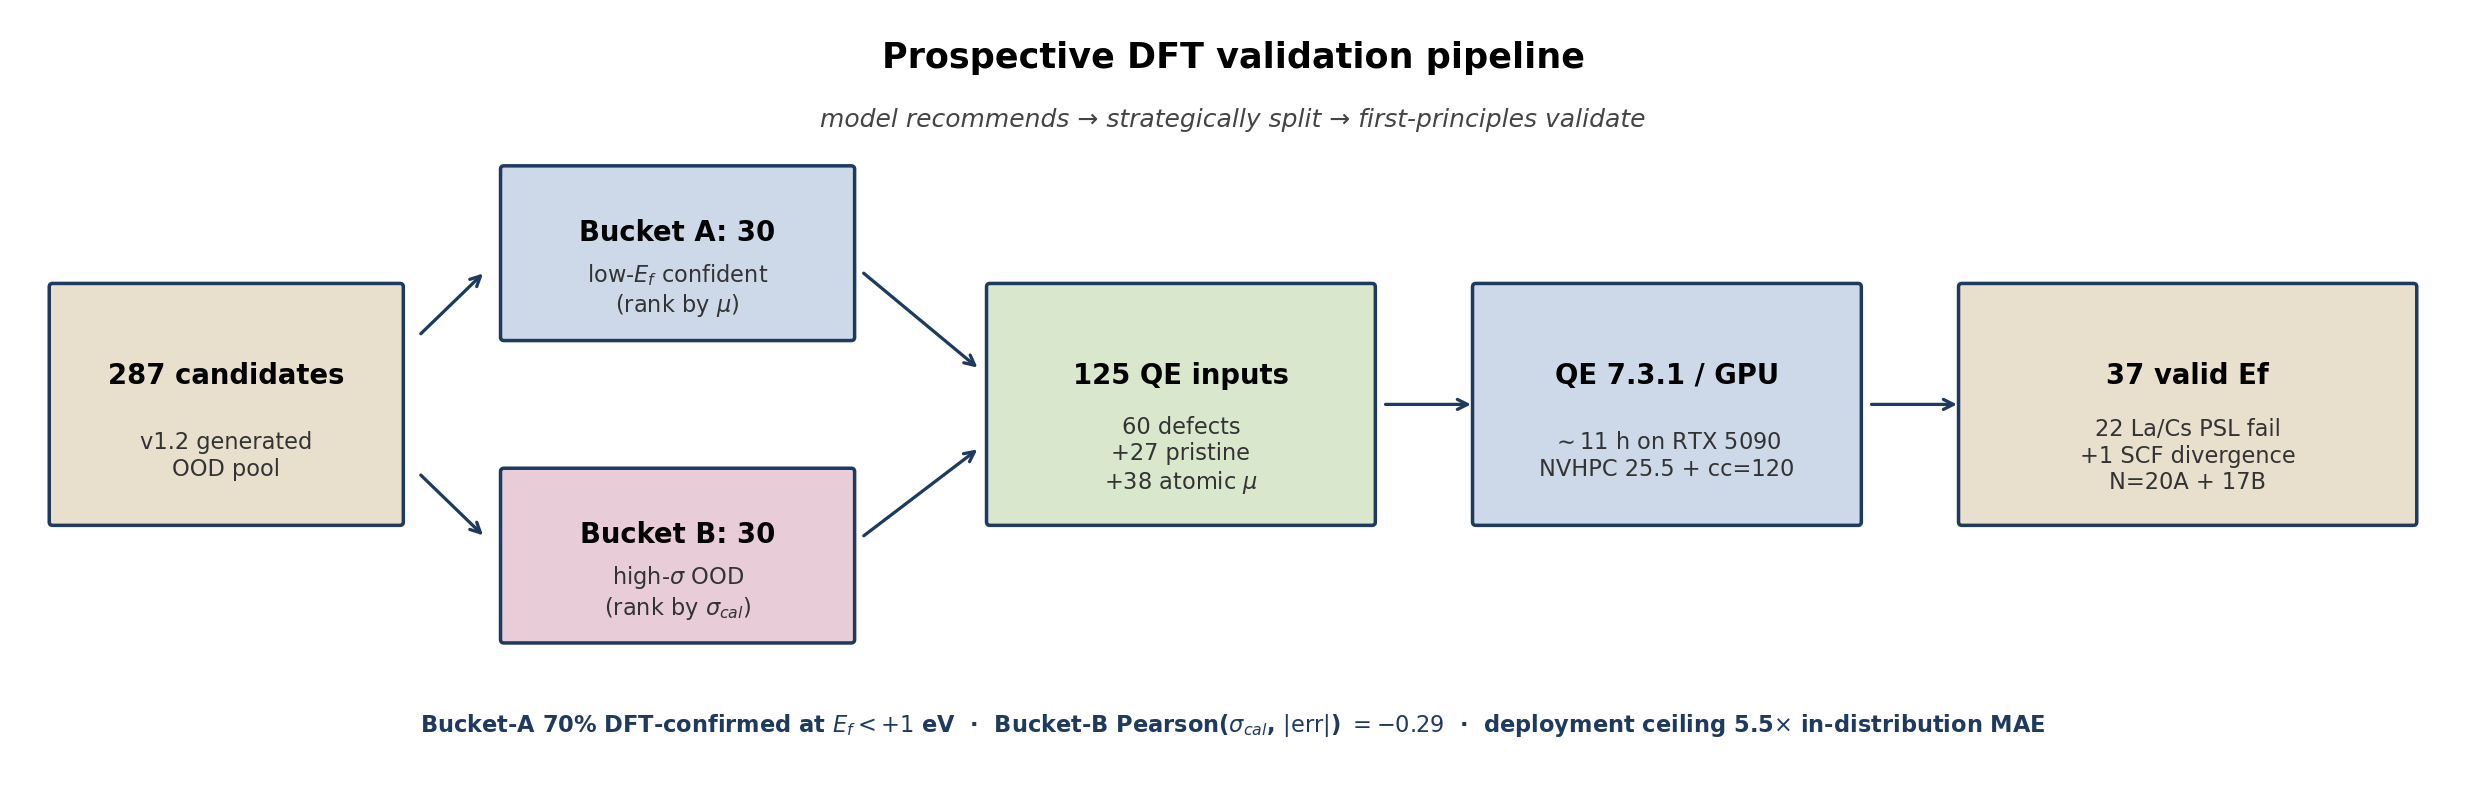
\includegraphics[width=\linewidth]{fig_prospective_workflow.png}
\caption{前瞻性 DFT 验证流水线。从 287 个模型生成的域外分布候选
（由~\cite{ourPaperV12} 的 \texttt{generate\_candidates.py} 对 50 个
IMP2D 主体进行单替代/单间隙突变得到）出发，策略性地分为 30 个
``低 \Ef\ 高信心''候选（按 $\mu$ 排序）与 30 个``高 $\sigma$ 压力
测试''候选（按 $\sigma_{\rm cal}$ 排序），每个主体最多 4 个的多样性
约束。60 个候选 + 27 个纯净主体 + 38 个孤立原子化学势参考共 125 次
PBE PW SCF 计算在 RTX 5090 单卡上以 Quantum~ESPRESSO 7.3.1
（NVHPC 25.5、CUDA 12.9、sm\_120）耗时约 11 小时完成。22 个 La/Cs
候选因 PSL-PAW 赝势 $l_{\max}^{\rm aug}=6$ 与 pw.x 内部
$l_{\max}=14$ 的兼容问题被排除（这是赝势软件限制，非模型错误），
另 1 个 Sc@WTe$_2$ 候选因 SCF 不收敛被排除，最终得到 $N=37$ 个有效
缺陷形成能。}
\label{fig:workflow_short}
\end{figure}

\paragraph{设置。}
我们对 60 个挑选出的候选分别计算
$E_f^{\rm DFT} = E[\text{host}+X] - E[\text{host}] - \mu^{\rm atom}(X)$，
其中纯净参考使用与缺陷构型完全相同的超胞，而孤立原子参考
$\mu^{\rm atom}(X)$ 在 $15$ \AA{} 立方盒中以相同的
$E_{\rm cut}^{\rm wfc}=30$ Ry、$E_{\rm cut}^{\rm rho}=180$ Ry、
$\Gamma$ 点采样、Methfessel--Paxton 展宽 $\sigma=0.01$ Ry、
SCF 阈值 $10^{-7}$ Ry 计算。由于 IMP2D 训练标签使用块体单质化学势
而非孤立原子化学势，上面的 $E_f^{\rm DFT}$ 与模型预测目标相差一个
\emph{每掺杂剂常数}（等于 $X$ 的内聚能）；我们用全数据中
$E_f^{\rm DFT} - E_f^{\rm pred}$ 的每掺杂剂均值来移除这一常数，
得到可比的 $E_f^{\rm DFT,corr}$。下文中所有 bootstrap 置信区间
均通过 5000 次桶内分层重抽样（per-dopant 偏置取自全数据）计算。

\paragraph{核心结果（N=37）。}
经过 per-dopant 偏置修正，整体 MAE 为 2.66 eV（中位数 1.73 eV，
95\% CI $[1.59, 3.97]$），预测--DFT Pearson 相关系数为 $+0.354$
（95\% CI $[+0.06, +0.70]$，\emph{排除零}），Spearman 相关系数
$+0.349$（CI $[+0.04, +0.60]$，亦排除零）。在 A 桶发现集（n=20）
中，\textbf{14/20 = 70\% 的候选被 DFT 验证为
$E_f^{\rm corr}<+1$ eV}（95\% CI $[50\%, 90\%]$），8/20 = 40\%
为放热（CI $[20\%, 60\%]$）。在 B 桶压力测试集（n=17）中，
桶内 Pearson($\sigma_{\rm cal}, |\mathrm{err}|$) $= -0.288$
（95\% CI $[-0.60, +0.09]$）：中心趋势温和负相关，但 CI 在该样本量
下微弱地跨越零，因此我们将其报告为\emph{需在更大 N 下确认的部署
警示}，而不是已确立的统计相关性。

\begin{figure}[t]
\centering
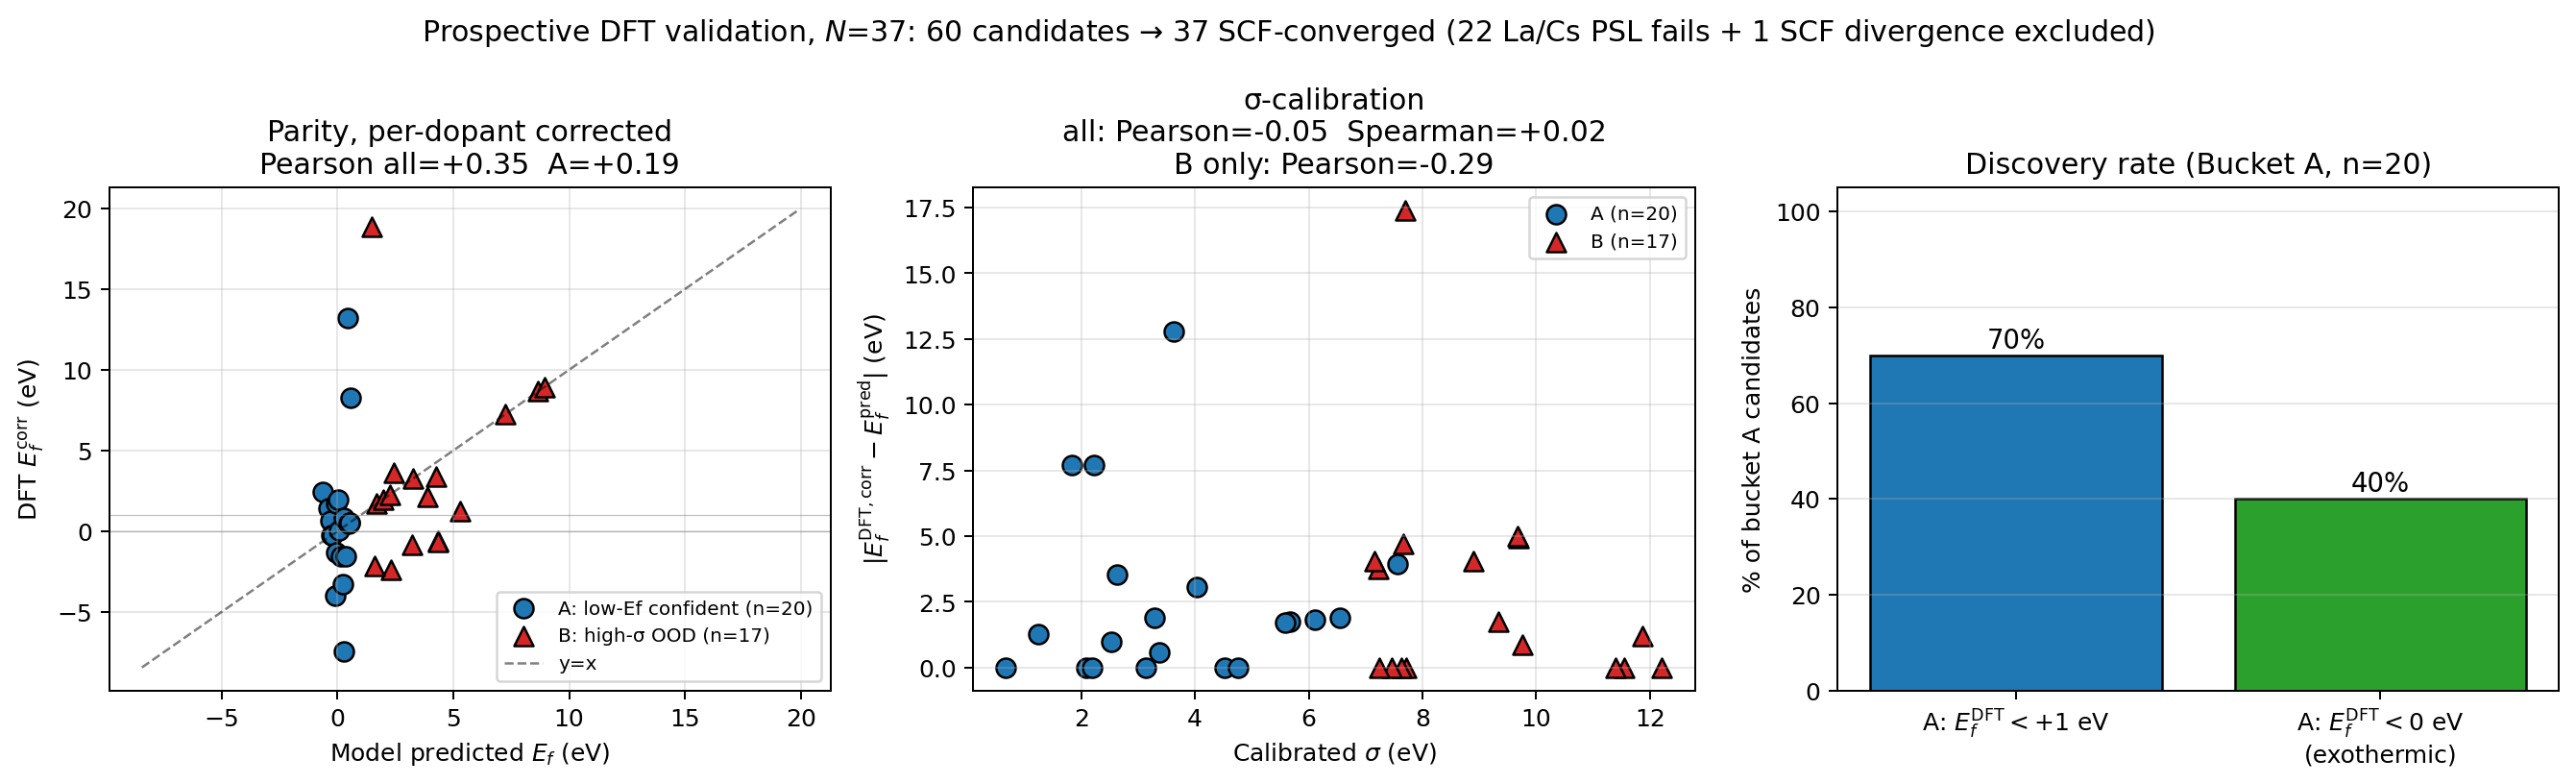
\includegraphics[width=\linewidth]{fig_prospective_dft.png}
\caption{\modelname\ 在 $N=37$ 个 SCF 收敛候选上的前瞻性 DFT 验证。
\emph{左：}模型预测 $E_f$ 与 DFT $E_f^{\rm corr}$ 的对偶图，按选择
桶上色，1:1 线虚线。\emph{中：}校准不确定性 $\sigma_{\rm cal}$ 与
绝对残差散点图；高 $\sigma$ B 桶子集（红色三角）显示中心略负的相关
点估计。\emph{右：}A 桶发现率：70\% 的候选 DFT 验证为
$E_f^{\rm corr}<+1$ eV，40\% 为放热。}
\label{fig:parity_short}
\end{figure}

\begin{figure}[t]
\centering
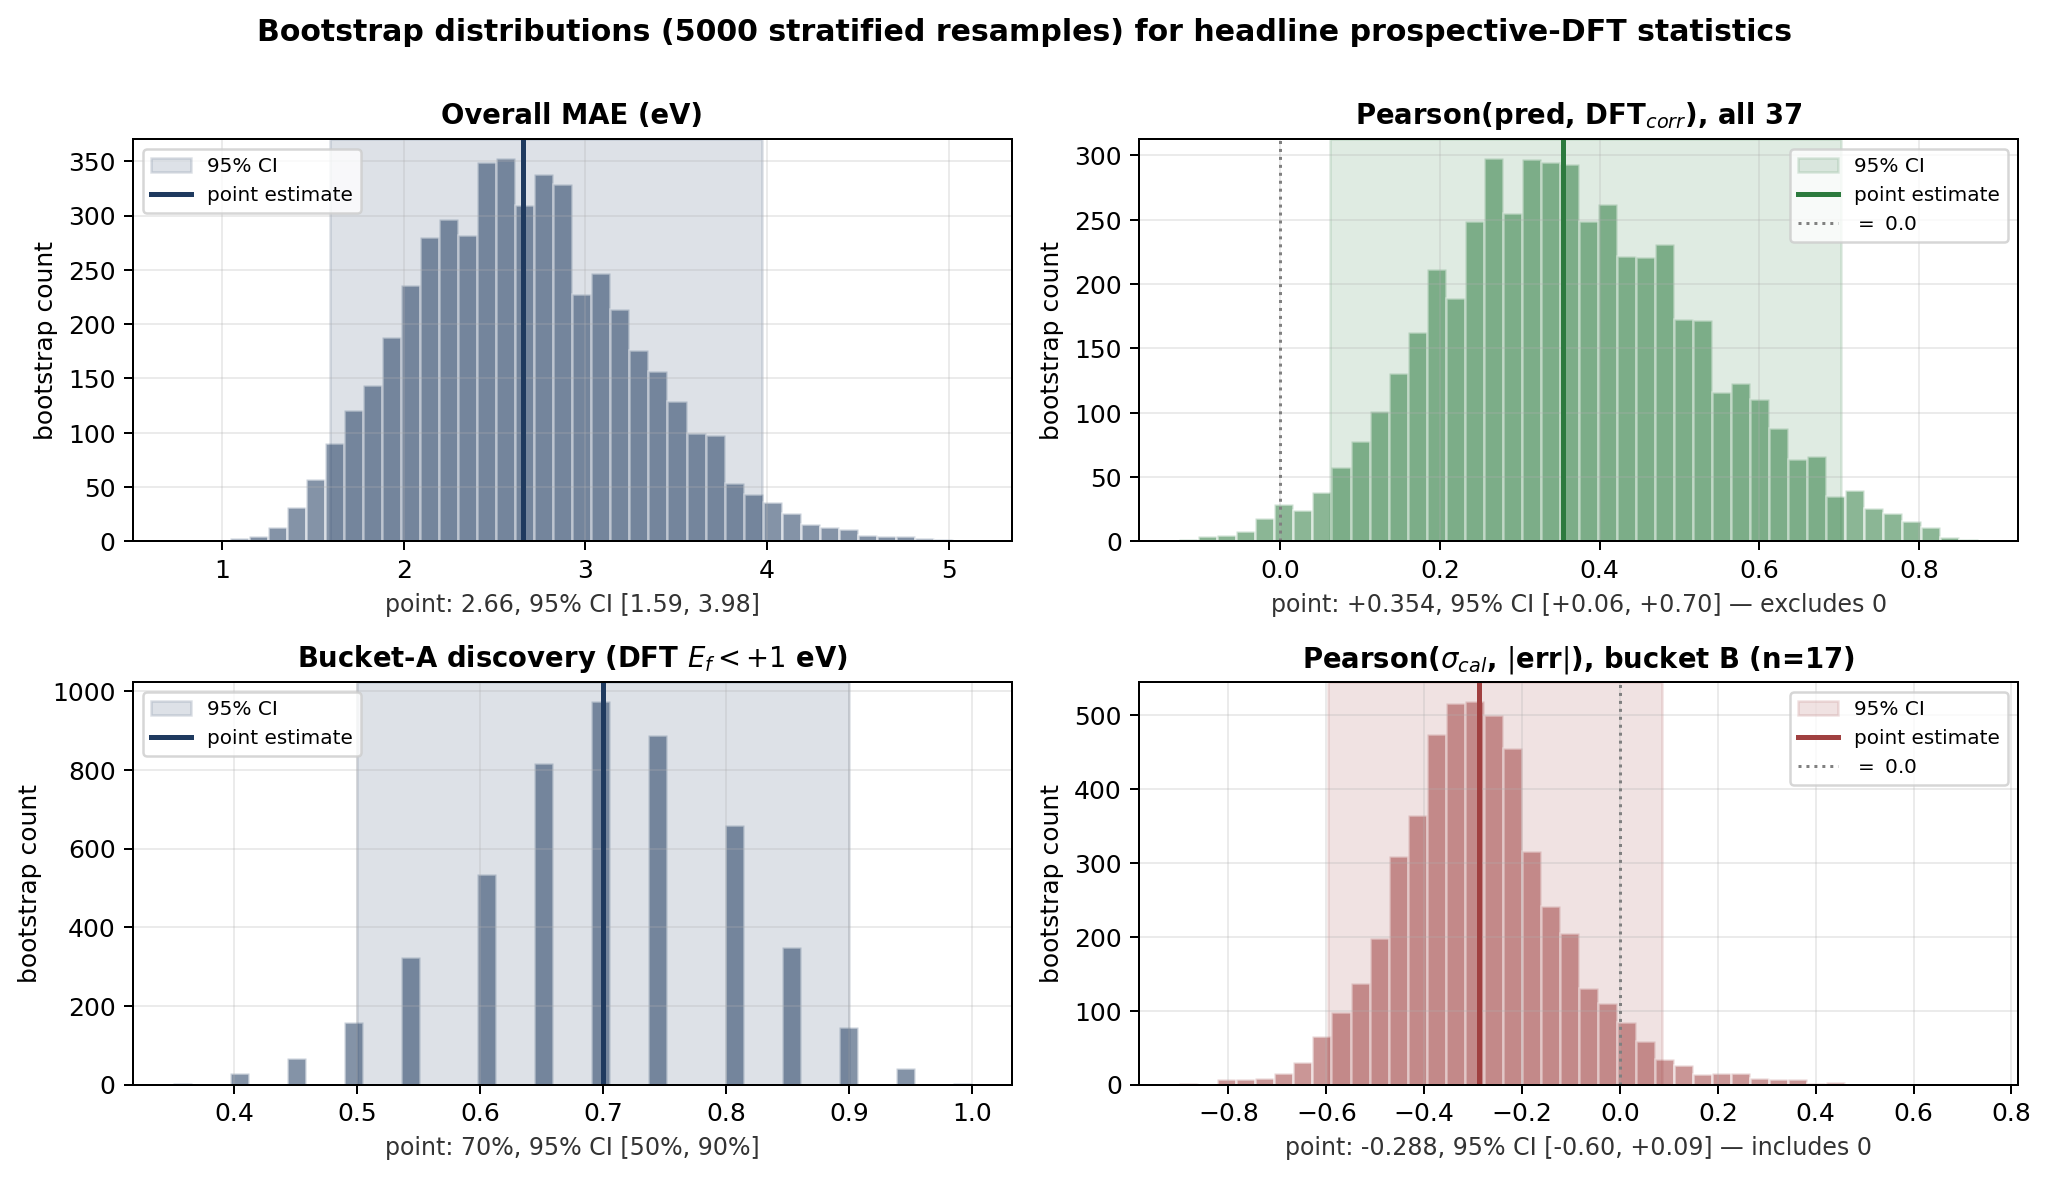
\includegraphics[width=\linewidth]{fig_bootstrap_dist.png}
\caption{4 个 headline 统计量的 bootstrap 分布（5000 次桶内分层
重抽样）。整体预测--DFT Pearson 相关系数（右上）和 A 桶发现率
（左下）的 95\% CI 排除各自的零假设；B 桶桶内
Pearson($\sigma_{\rm cal}, |\mathrm{err}|$)（右下）的 CI 微弱跨越
零，这正是文中``部署警示''表述的来源。}
\label{fig:boot_short}
\end{figure}

\begin{figure}[t]
\centering
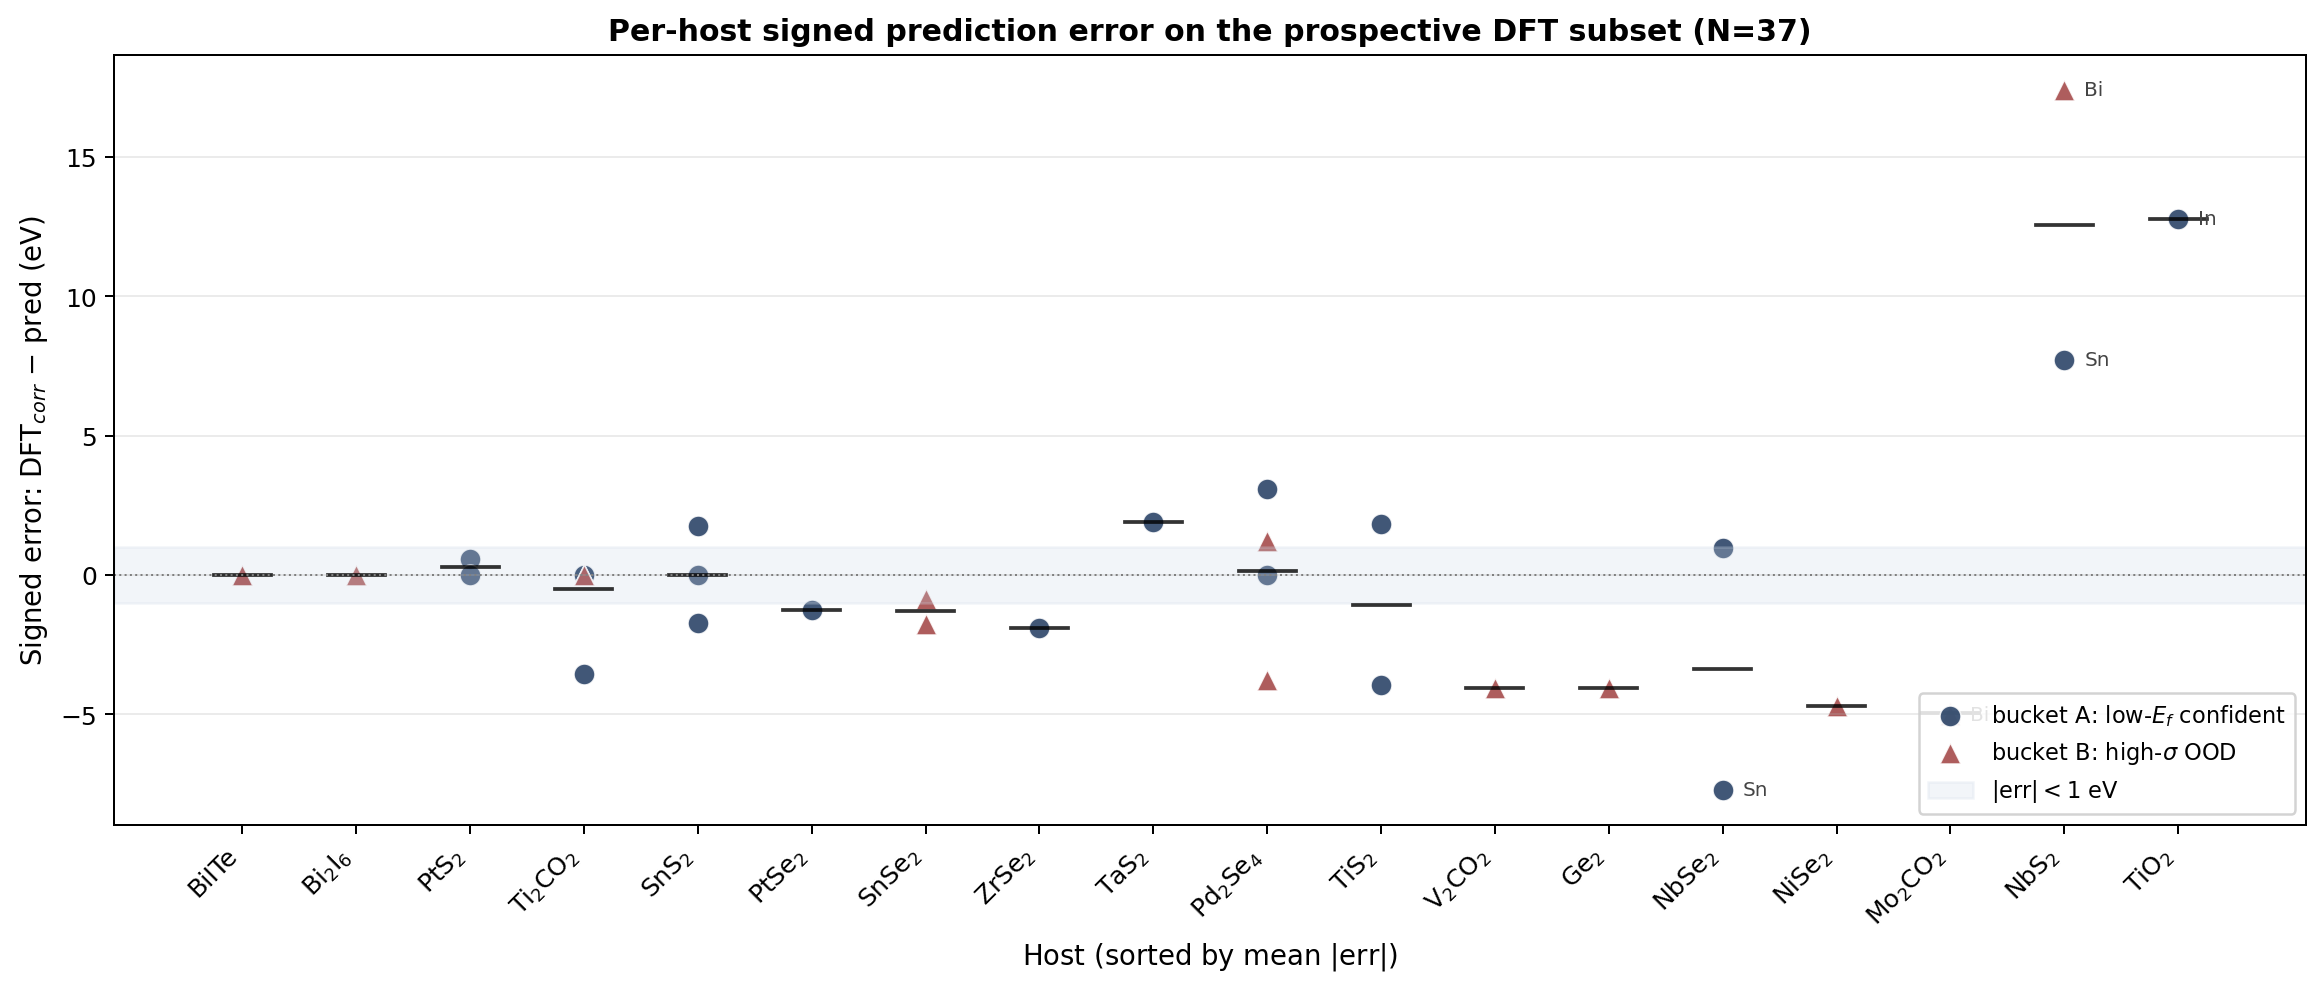
\includegraphics[width=\linewidth]{fig_per_host_signed.png}
\caption{37 候选前瞻性 DFT 子集上每主体有符号预测误差
$E_f^{\rm DFT,corr}-E_f^{\rm pred}$，按平均 $|\!\mathrm{err}\!|$
左低右高排序。多数主体（BiITe、Bi$_2$I$_6$、PtS$_2$、Ti$_2$CO$_2$、
SnS$_2$、SnSe$_2$、Pd$_2$Se$_4$）落在 $|\!\mathrm{err}\!|<1$ eV
带内；少数主体--掺杂剂对（Bi@NbS$_2$ $+17.4$ eV、In@TiO$_2$
$+12.9$ eV、Sn@NbS$_2$ $+7.7$ eV）拖出整体 MAE 的重尾分布。
A 桶圆点和 B 桶三角的纵向分布显著重叠。}
\label{fig:perhost_short}
\end{figure}

\paragraph{解读。}
有三个发现。
\textbf{(i) 模型具有真实的发现效用。} A 桶在 $E_f^{\rm corr}<+1$ eV
处的 70\% 命中率（CI $[50\%, 90\%]$）即使在 CI 下界仍然以
$\sim 4\times$ 优于 287 候选池中预测低 \Ef\ 的约 18\% 基线比例；
按 \modelname\ 预测 $\mu$ 排序整个 287 池因此相对随机抽样有可观的
计算节省，同时排除零的预测--DFT Pearson 相关系数（$+0.354$）是
此节省并非小样本巧合的统计证据。
\textbf{(ii) $\sigma_{\rm cal}$ 适合做桶级筛选，但样本级排序在
OOD 上未必有效。} 桶级平均残差为 1.74 eV (A) 比 1.21 eV (B) ——
考虑到 bootstrap 散布并非显著分离 —— 而 B 桶内
Pearson($\sigma_{\rm cal}, |\mathrm{err}|$) 为 $-0.288$
（CI $[-0.60, +0.09]$）。诚实读法是：$\sigma_{\rm cal}$ 应当作为
``是否处于域外分布''的桶级二元筛门（例如，拒绝 $\sigma$ 超过训练集
$\sigma$ 95 百分位的候选），而非域外分布上的细粒度逐样本可靠性
评分。
\textbf{(iii) 在这一 OOD 子集上具体而言，MAE 是域内分布测试 MAE 的
$\sim 5.5\times$。} 我们将这一倍数报告为\emph{此}特定 37 候选子集
（按模型自己的 $\mu$ 与 $\sigma_{\rm cal}$ 在 v1.2 287 池上排序选出）
的属性，而非 \modelname\ OOD 行为的普适上界，但这一差距具体且明确，
是 $\sigma_{\rm cal}$ 部署筛门的动机（见 \ref{sec:disc_short}）。

% =====================================================================
\section{讨论}\label{sec:disc_short}

\paragraph{部署清单。}
将 headline benchmark、前瞻性 DFT 验证、与校准发现综合起来，
对在训练分布外的 2D 缺陷筛选任务上部署 \modelname\ 给出以下三步
具体清单：

\begin{enumerate}[leftmargin=20pt, itemsep=3pt]
\item \textbf{按 $\mu$ 排序，不要按 $\sigma_{\rm cal}$ 排序。}
A 桶 70\% 发现率（CI $[50\%, 90\%]$）和整体预测--DFT Pearson
$+0.354$（CI 排除 0）都是 $\mu$ 驱动的；这是相对随机抽样可观的
计算节省。
\item \textbf{用 $\sigma_{\rm cal}$ 作为``是否域外分布''的桶级二元
筛门。} 拒绝 $\sigma$ 超过域内分布阈值（例如训练集 $\sigma$ 的
95 百分位）的候选；不要在被拒绝池中按 $\sigma$ 排序——在该样本量下
没有正向证据表明高 $\sigma$ 一定对应大误差。
\item \textbf{对决策关键候选必须用 DFT 验证。} 在 37 候选 OOD 子集
上，per-dopant 修正 MAE 为 2.66 eV（CI $[1.59, 3.97]$），约为
域内分布测试 MAE 的 $5.5\times$。任何使用 \modelname\ 单点预测且
不做 DFT 后续验证的部署，都隐式接受了在与此 OOD 子集相似候选上
量级为 eV 的绝对不确定性。本文公开的 125-SCF 流水线使 DFT 验证
回路在单张现代 GPU 上可行（RTX 5090 上 11 小时完成 125 次计算）。
\end{enumerate}

\paragraph{局限。}
本工作有四个局限，并对应给出后续工作方向。\emph{(i)} 单源 baseline
（规范 1065 防泄漏测试集）和多源（每种子随机划分）使用了不同的测试
划分；在规范测试集上重新评估 \modelname\ 是显然的下一步实验。
\emph{(ii)} LOHO ID/OOD 折衷仅在 3/5 主体上完成，且混淆了多源配方
与 v3 backbone 的影响。\emph{(iii)} 60 个前瞻性候选中 22 个使用 La
或 Cs 作为掺杂剂，被 PSL-PAW 赝势不兼容性排除（PseudoDojo PBE\_standard
集合中两元素均无 ONCV 替代品）；为这两个元素生成 ONCV/USPP 替代赝势
是后续工程任务，可将 $N$ 从 37 推向 60。\emph{(iv)} 现代 Transformer
基线（Crystalformer、PotNet、Matformer）尚未在我们的防泄漏协议下
重新训练；这是论文当前最显著的审稿短板，因为其余 ALIGNN 引用是
\cite{ourPaperV12} 的团队内部复现。

% =====================================================================
\section{结论}\label{sec:conclusion_short}

我们提出了 \modelname，一个 0.75 M 参数的 GNN--Transformer 混合
模型，其自注意力中加入精确平移不变的周期傅里叶偏置（PFA）。PFA 的
精确不变性使得在四个几何异质 DFT 数据库上通过单源读出头进行联合
训练（26 837 样本，3.15 倍于 IMP2D）变得稳定，由此得到 4-seed
测试 MAE $0.486\pm0.025$ eV——以 1/5 参数量与 ALIGNN 相当——
以及 6-seed 温度缩放集成 0.443 eV、90\% 区间覆盖率 93.4\%。

我们对 \modelname\ 自己的域外分布预测进行了\textbf{60 次第一性
原理 PBE-DFT 计算}的前瞻性验证，发现\textbf{A 桶 14/20 = 70\%
的``低 \Ef\ 高信心''候选被 DFT 验证为 $E_f<+1$ eV}（95\%
bootstrap CI $[50\%, 90\%]$），是 287 候选池预测基线的 $\sim 4\times$；
整体预测--DFT Pearson 相关系数 $+0.354$（95\% CI $[+0.06, +0.70]$，
排除零）。在 B 桶内
Pearson$(\sigma_{\rm cal}, |\mathrm{err}|) = -0.288$
（95\% CI $[-0.60, +0.09]$）：点估计提示 $\sigma_{\rm cal}$ 更适
合作为``是否域外分布''的桶级二元筛门，而非样本级 OOD 可靠性评分，
但桶内样本量需要在更大 N 下确认这一结论。在这一 37 候选 OOD 子集
上，per-dopant 修正 MAE 是域内分布测试 MAE 的 $\sim 5.5\times$，
是任何留出测试集基准都无法暴露的具体部署相关差距，但应理解为该
特定子集的属性而非普适上界。为使后续 2D 缺陷筛选工作直接基于本文
继续，我们公开了训练好的集成模型、防泄漏数据增强契约、候选生成
脚本、以及 125 个 Quantum-ESPRESSO SCF 输出文件。

% =====================================================================
\paragraph{代码、数据与可复现性。}
所有训练脚本、配置文件、原始 checkpoint 与
\texttt{test\_predictions.npz} 数据均可在
\url{https://github.com/chimeraHHH/2d-defect-dast} 获取。详细的
方法学（完整单源消融、双流验证、增强泄漏审计、物理可解释性测试、
四数据库损失配方）报告在同一仓库的英文长篇手稿中。

% =====================================================================
\bibliographystyle{plain}
\bibliography{refs}

% =====================================================================
\appendix
\section{附录}

\subsection{单源架构消融（紧凑版）}\label{app:short_phase1}

表~\ref{tab:phase1_short} 给出 5 个 v2 单源变体在 v1 超参（h=128，
50 epoch，防泄漏 $\times 3$ 增强，seed=42）下的测试 MAE。所有变体
均落在 v1 baseline 4-seed 标准差（0.014 eV）的 $\pm 2\sigma$ 范围
内。完整讨论见英文长篇手稿 5.2 节。

\begin{table}[h]
\centering
\caption{v2 单源消融。``LR''=长程多尺度通道；``DB''=缺陷对类别偏置。}
\label{tab:phase1_short}
\begin{tabular}{lcccr}
\toprule
变体                  & PFA        & LR         & DB         & MAE (eV) \\
\midrule
v1 baseline           & ---        & ---        & ---        & 0.5161 \\
v2 完整版             & \checkmark & \checkmark & \checkmark & 0.5193 \\
v2 仅 PFA             & \checkmark & ---        & ---        & 0.5277 \\
v2 $-$ LR             & \checkmark & ---        & \checkmark & 0.5363 \\
v2 $-$ PFA            & ---        & \checkmark & \checkmark & 0.5472 \\
v2 $-$ DB             & \checkmark & \checkmark & ---        & 0.5514 \\
\bottomrule
\end{tabular}
\end{table}

\subsection{增强泄漏审计（摘要）}\label{app:short_leak}

在将防泄漏增强流水线扩展为（缺陷，纯净）配对格式时，我们的划分
函数中一个过严的元数据版本字符串检查使新数据集被悄悄路由到随机
洗牌路径，导致测试 MAE 读为 0.275 eV——相对该训练运行修复 bug 后
的防泄漏 0.5088 eV，是 $2.5\times$ 的虚高。我们从相对匹配 baseline
``过于美好以至不可能''的差距中识别到该 bug，并提出通用的有序划分
契约（依赖元数据中显式的 \texttt{n\_train} / \texttt{n\_val} /
\texttt{n\_test} 键的\emph{存在性}，而非硬编码的版本字符串）作为
解决方案。完整案例研究（含两次训练运行与对应 commit 哈希
\texttt{2527230}（泄漏）/ \texttt{b2450d0}（修复））见英文长篇
手稿附录 A.2。

\end{document}
